\documentclass{article}
\usepackage[utf8]{inputenc}
\usepackage{graphicx}
\graphicspath{ {images/} }
\usepackage{amsmath}
\usepackage{gensymb}
\usepackage[english]{babel}
\usepackage[version=4]{mhchem}
\usepackage[T1]{fontenc}
\usepackage{wrapfig}
\usepackage[colorlinks,citecolor=blue,urlcolor=blue,linkcolor=blue, bookmarks=false,hypertexnames=true]{hyperref} 
\usepackage[font=scriptsize,labelfont=bf]{caption}
\usepackage{subcaption}
\usepackage[backend=biber,style=authoryear-comp]{biblatex}
\usepackage[a4paper, portrait, margin=1in]{geometry}
\addbibresource{mybib_stable.bib}

\setlength{\parindent}{4em}
\setlength{\parskip}{1em}
\renewcommand{\baselinestretch}{1.5}

% \title{GIS For Dummies: Live Demonstration Guide}
% \author{Nicholas D. Barber}
% \date{\today}

\begin{document}

\begin{titlepage}
   \begin{center}
       \vspace*{1cm}

       \LARGE
       \textbf{GIS For Dummies: Session 2 Live Demo Guide}
       
       \Large
       \vspace{0.3cm}
        GIS Workshop prepared for McGill University Society for Economic Geology Student Chapter
            
       \vspace{1.2cm}
       \textbf{Nicholas D. Barber}\\
       Department of Earth Science\\
       University of Cambridge\\
       United Kingdom\\
       June 22nd, 2020
            
       \vspace{0.8cm}
     
       \includegraphics[width=0.9\textwidth]{Figure1_HazardMap_GP.png}
   \end{center}
\end{titlepage}

\tableofcontents

\section{Course Overview}

This guide was written in June of 2020 as an accompaniment to the "GIS for Dummies" workshop, organized by Catherine Crotty and Saraha Bodeving of McGill University (Canada). The workshop was presented in four parts, with the aim of introducing the use of Geographic Information Systems (GIS) to geoscientists in McGill's Society for Economic Geology (SEG) chapter. This section will provide a more general overview of the workshop, and preview the structure of the following guide, which is meant to accompany Part 2, Exercise 1. \textbf{All contents of this guide have been prepared by the course instructor, Nicholas Barber, and this guide can be shared under a MIT Shared Software License.} Feel free to share this guide and accompanying resources! \textit{Disclaimer: I (Nick Barber) claim no ownership of the data or underlying software used in this guide or this course.} 

This workshop was setup after preliminary discussions between myself, Catherine and Sarah throughout May 2020. In their role as organziers for their SEG chapter, they articulated a need to showcase what GIS is and what it can do for geoscientists. They wanted this course to include both a crash course for beginners, while also showcasing advanced features for more experienced users. Given the ongoing pandemic, the course was also to be hosted virtually. With these parameters in mind, I wrote an outline dividing our time into 4 blocks, to be spread over 4 days. Session 1 (Monday, June 15th) gave an overview lecture, covering the motivation for the course (Section XX), my background (see my web page), and the key theoretical material. The latter point as covered briefly, but ideally this topic will be given closer attention in a follow up GIS theory guide (this is a note to myself to write that, potentially for my undergrads). Wednesday June 17th saw Session 2, which in addition to this guide included a Lecture and a Live Demonstration of basic QGIS 3.10 functionality. The map on the title page is the desired output from Session 2. Session 3 will take place on Monday June 29th. The goal in this 2 hour block will be to run through some more advanced material, covering Python, spatial databases, mineral exploration (?) and style. Session 4 will be an open day where participants can schedule 1-1 thirty minute blocks with me, where I will advise them on their projects and the ways to get going with their particular analyses in GIS. 

The following sections will summarize Exercise 1, providing pictures with step by step details on how to replicate what I did in the live demo. I will start by briefly highlighting some of the goals and target skills in this demo. 

\subsection{Objectives}

The goal of this exercise to to familiarize users with the work flow of a typical GIS project.I wanted to show in (mostly) real time how you conceptualize a problem, find the data, set up the QGIS environment, conduct analyses, and export your desired output. I want this exercise to be both (1) an introduction to GIS project management and basic GIS analyses for users who may have never opened the program before, and (2) a refresher on basic GIS tasks, menus, and tools for more experienced users. \textbf{My hope is that whether you are a new or returning GIS user, you leave this workshop with a fuller appreciation of the functionality of GIS and the applications of GIS in geological research.} 

Our research question for this exercise: \textbf{How many people are at risk to the different eruptive products of Guagua Pichincha Volcano, Ecuador (\href{fig:fig1}{Figure 1})?} I selected this question for a few reasons. The first reason is that, on the whole, this question is pretty easy to answer using GIS. This is because the datasets required are quite readily available, and require minimal manipulation to get in a use able form. However, the challenge of this project is the fact that it requires non-geological data which geologists are often loathe to find. It also takes place in an area of the world many people in the McGill SEG chapter may be unfamiliar with, and the metadata is even in another language! Further complicating things is that the geological information available is locked away in non-georeferenced datasets. So while this question is easy to address at a birds eye view, if you want to answer it \textbf{you need the a full appreciation of the core "GIS Toolkit," which is the goal of this course.}

\begin{figure}[htbp]
    \centering
    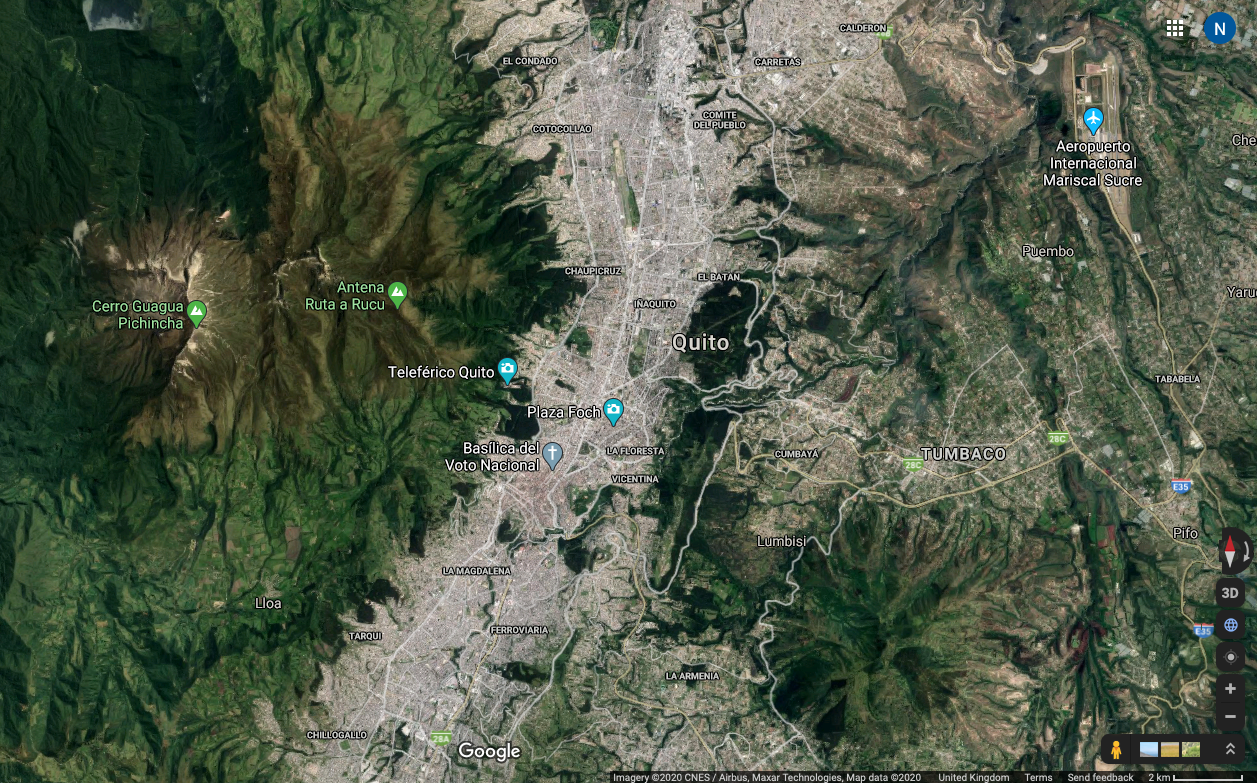
\includegraphics[width=0.8\textwidth]{Google Map Overview of GP and Quito.png}
    \label{fig:fig1}
    \caption{Screen shot of Guagua Pichincha, looking North with Quito, capitol city of Ecuador, dominating the lowlands to the East. Image taken from Google Maps on June 23rd, 2020. }
\end{figure}

\subsection{Transferable Skills}

Based on these goals, Exercise 1 should impart several important skills that will be useful in any GIS project:

\begin{itemize}
  \item Project Planning
  \item Locating Data and Understanding Metadata
  \item Importing Data
  \item Setting Up a QGIS Workspace
  \item Defining a Coordinate References System (CRS) and Projected Coordinate System (PCS) for your Project
  \item Reprojecting Data
  \item Georeferencing a Base Map
  \item Calculating Errors
  \item Geoprocessing
  \item Spatial Statistics
  \item Styling Raster and Vector Data
  \item Visualizing Geographic Data
\end{itemize}

\section{Project Panning + GIS Motivation}

The first topic addressed in the lecture was the need to properly articulate WHY you need GIS, and WHAT you intend to get out of a GIS analysis. This is similar to any self-directed critical question you'd ask yourself in research, e.g. "what am I hoping to achieve with this particular tool?" The reason I want to be up front about this need is because like any other research technique, GIS involves training, and you want to be sure the time invested in using GIS is invested wisely. Some of the operations I show you in this guide can be performed in other software suites - particularly using Python and R. If your goal is limited in scope, it might be worthwhile to see if any of your other skill-sets will allow you to answer the same question. 

With that preface in mind, there are several obvious reasons why you might plan a project with GIS in mind. When you want to take a range of spatial datasets, overlay them, analyze some feature(s), and produce a well defined, beautiful map, Python's command line (or cell-by-cell interface in case of an IDE like Jupyter Notebook) may not be the most logical and effective way to structure your project. One of the clear advantages of GIS software is its interface, which allows the user to control every aspect of the data in question, most especially its appearance. This interface is at the same time a big barrier for people getting into GIS - the first time you open QGIS, you'll be overwhelmed by the sheer number of menus, buttons, and tools at your disposal. This is where time investment, mentioned in the previous paragraph, really comes in. In my experience, half the battle in a GIS project is finding the right button or menu, which is often buried in some obscure interface. But the fact that there are so many ready-made tools and options in a software like QGIS adds to the value of the software. Rather than defining a spatial analysis procedure from scratch and formatting the resultant map using something like \textit{matplotlib}, GIS lets you does a lot of the background work for you. 

Another advantage of a GIS is its ability to contextualize your data. Say you are a geochemist, and you've spent months in the lab analyzing a suite of elements in your samples. After all that hard work, you will naturally want to extract the maximum scientific value out of your results. This can of course be done without a GIS, but as we shall see, overlaying your spatially-defined sample data with GIS layers describing the natural hazards, topography, hydrology, and demography in your study area can provide a much richer picture of the impact your results on the systems + people it comes from. If you had analysed whole rock chemistry of scoria from different eruptive periods at Guagua Pichincha, or modeled the record of earthquakes below the edifice over a long time period, you will be able to say with certainty what impact the hazard you've identified will have on the populations affected. This analogy extends beyond volcanology of course; you should be able to see the same spatial dimension in any geological dataset, and as soon as that dimension is visualized the apparent usefulness of GIS should jump out. Finally, I can't end this discus ion without highlighting the power of GIS to advance your career. In the private and public sector, having a GIS skill set marks you out as a great candidate for a host of jobs both in the field and in the office. Given the time and experience it takes to master GIS workflows, companies and organizations will value you for this skill, which is applicable well outside geology. In fact, GIS is arguably more important than many highly technical geological skills we learn in a PhD, as they are applicable in some many non-academic applications: think Google maps, software development, COVID tracking, environmental remediation, hydrogeology, subsurface exploration, etc. 

Having laid out all these considerations as to WHY you might choose to sue a GIS, the next logical step is to ask: "Where do I start?" The first point for any scientific investigation is your research question. Thanks to the discussion in the previous section, we already have that established in our case. It's worth adding that this question comes to us because Guagua Pichincha is only 10 km. W of Quito, the capitol of Ecuador. Depending on the nature of the hazards posed, we can hypothesize a large proportion of the population are under threat from this volcano. Our next step after framing our question is to think about what stage of our analysis GIS will factor into. GIS is incredibly helpful when planning field work, as the mapping functions should make obvious. However, GIS can also add that "context" to your data I mentioned before. Even if you don't need to do any exploration or data, the map-making functionality alone makes GIS essential for manuscript figure generation. Based on these features, we can break the "stages" of GIS applicability into a \textbf{Early Stage} (planning, querying available data, generating a research question), \textbf{Analysis Stage} (spatial statistics, validating analyses, contextualizing results, modeling), and a \textbf{Post-Analysis Stage} (figure creation, map making, preparing data for publication).  

Once we have the WHY and the WHERE, we need the WHAT and HOW: what specific steps and information do you need to set off on this project. This guide will examine the search for data and the specific steps for GIS analysis in great detail. However, two more factors can be brought into our project plan. The first is follows on from my lecture in Session 1, and that's the coordinate/projection system we are going to use. This will also be treated in some detail below, but regardless of which stage of GIS analysis you are in, this needs to be one of the first things thought about and decided upon. For now, we will put a pin in that as we search for the data we need and get our GIS work space set up for the first time. The second factor is something that comes with experience, and that's an early "sketch," of the steps we will need to take in our project. For example, I know looking at our research question, I'll essentially need to compare the areas of two vector files: the vector file describing the spatial footprint of the hazard, and the vector file describing the spatial distribution of the population. This operation is called an \textbf{Overlay} and can be accomplished with several different \textbf{Geoprocessing} tools, all with applicability in different situations. Like anything else, this forecasting of the tools needed to answer our questions only comes with practice. I'll share some more thoughts on this topic at the end of this document. However, for now, we are ready to begin our GIS journey. 

\section{Downloading and Installing Software}

\section{Finding GIS Data}

\section{Importing Data}

\subsection{Vector}

\subsection{Raster}

\subsection{CSV}

\section{Defining Coordinate Systems and Projections}

\subsection{Reprojection}

\section{Setting Up Workspace}

\section{Georeferencing Our Base Map}

\section{Creating New Features}

\section{Accounting for errors}

\section{Analysis}

\subsection{Field Calculator}

\subsection{Geoprocessing}

\subsection{Statistics Viewer}

\section{Symbology}

\subsection{Vector}

\subsection{Digital Elevation Models (DEMs)}

\subsection{3D View}

\section{Creating a Map: Layout Manager}

\section{Final Thoughts}

\section{Data Sources and Further Reading}

\section{Acknowledgements}

\newpage
\printbibliography

\end{document}
